\FloatBarrier
\subsection{Search after measured finalist improvement}
\label{app:public-stock-mature-variants}
The failed control qualification leaves the all-improved-policy study
unexecuted. A separate, prospectively fixed study retains original control
and tests both qualified finalists against the other improved parent.
Control has 128 adaptation updates and the finalists 512; original parent
training is reused separately. This unequal allocation precludes a
matched-training estimate of a rule effect. Within each rule, all search
budgets use the same actor and opponent. Rollouts and continuation values
still use the searching actor's own policy, without an opponent oracle or
access to actual hidden cards.

Four new policy-specific continuation tables require 1,933,312 conditional
round rollouts and 53,080,083 transitions. Independent reduction checks all
saved targets and means; fixed-stratum Python replay checks 15,104 rounds
and 415,656 decisions. The two original control tables are reused unchanged,
with identities and audit receipts checked. Their historical preparation is
not counted as new work. These sampled tables are not certified value bounds.

Work calibration uses two separate cohorts of 64 duplicate streams, both
seats. Initial measurements at 32 worlds propose low/high counts for targets
of 60,000/240,000 physical transitions per match. A second cohort measures
each proposed count and permits exactly one work-only correction. Both steps
round $tMp/T$ half-up and clamp to $[2,256]$, where $t$ is the target,
$M$ the matches, $p$ the measured world count and $T$ recorded transitions.
Independent reduction reproduces both stages before counts are frozen.
Calibration uses 768 then 1,536 matches, 121,172 then 241,350 scored/replayed
decisions, and 109,732,789 then 229,692,761 planning transitions. No outcome
selects a rule, checkpoint or budget. The final counts are in
Table~\ref{tab:public-stock-mature-costs}.

Reserved evaluation uses 256 new duplicate streams shared by all arms,
both seats, three rules, two parents and zero/low/high budgets: 9,216 matches,
65,435 rounds and 1,473,646 scored decisions. All decisions pass Python
replay; independent reduction reproduces outcomes, counts and identities.
Recorded search work is 66,947,471 rollouts and 926,858,779 transitions across
480,132 roots; these internal planning counters are not independently replayed.
The independent units are the 256 streams, not the number of matches.

Fourteen prespecified contrasts use 20,000 paired-stream bootstrap replicates
and two-sided quantiles $0.05/28$ and $1-0.05/28$, a nominal within-study
95\% familywise target. Each finalist requires positive lower bounds for
high-minus-zero, excess over retained control and high-minus-low, for both
parents. Ranking requires both finalist gain-difference intervals to exclude
zero in the same direction.

\begin{table}[ht]
\centering\small
\begin{tabular}{lllrrr}
\toprule
Rule & Parent & Comparison & Mean & Lower & Upper \\
\midrule
Preview + choice & 0 & High--zero & +25.68 & +19.14 & +32.23 \\
Preview + choice & 0 & Excess over control & +24.80 & +17.09 & +32.52 \\
Preview + choice & 0 & High--low & +9.86 & +4.39 & +15.33 \\
Preview + choice & 1 & High--zero & +26.76 & +20.51 & +33.20 \\
Preview + choice & 1 & Excess over control & +27.15 & +19.24 & +35.25 \\
Preview + choice & 1 & High--low & +11.91 & +5.96 & +17.97 \\
All three & 0 & High--zero & +25.78 & +19.14 & +32.62 \\
All three & 0 & Excess over control & +24.90 & +17.29 & +32.45 \\
All three & 0 & High--low & +9.96 & +3.03 & +16.89 \\
All three & 1 & High--zero & +28.42 & +22.07 & +34.60 \\
All three & 1 & Excess over control & +28.81 & +21.29 & +36.16 \\
All three & 1 & High--low & +10.45 & +4.20 & +16.70 \\
Preview + choice minus all three & 0 & Gain difference & -0.10 & -9.21 & +8.79 \\
Preview + choice minus all three & 1 & Gain difference & -1.66 & -10.35 & +7.23 \\
\bottomrule
\end{tabular}

\caption{All fourteen stronger-finalist comparisons in percentage points,
with simultaneous paired-bootstrap intervals under the fixed V5C family.
Excess subtracts retained control's corresponding high-minus-zero gain.
The last two rows compare search gains, not absolute strength across games.
Scores count ties as one half.}
\label{tab:public-stock-mature-comparisons}
\end{table}

Both finalists pass all six score inequalities. Preview plus choice gains
25.68/26.76 points over zero search; all three gains 25.78/28.42 points.
Increasing low to high adds 9.86/11.91 and 9.96/10.45 points, respectively,
with every simultaneous lower bound positive. The retained control's
high-minus-zero means are $+0.88/-0.39$ points. Thus the computation benefit
persists after measured finalist improvement and against another improved
parent; it is not restricted to the earlier, weaker adapted actors.

\begin{figure}[ht]
\centering
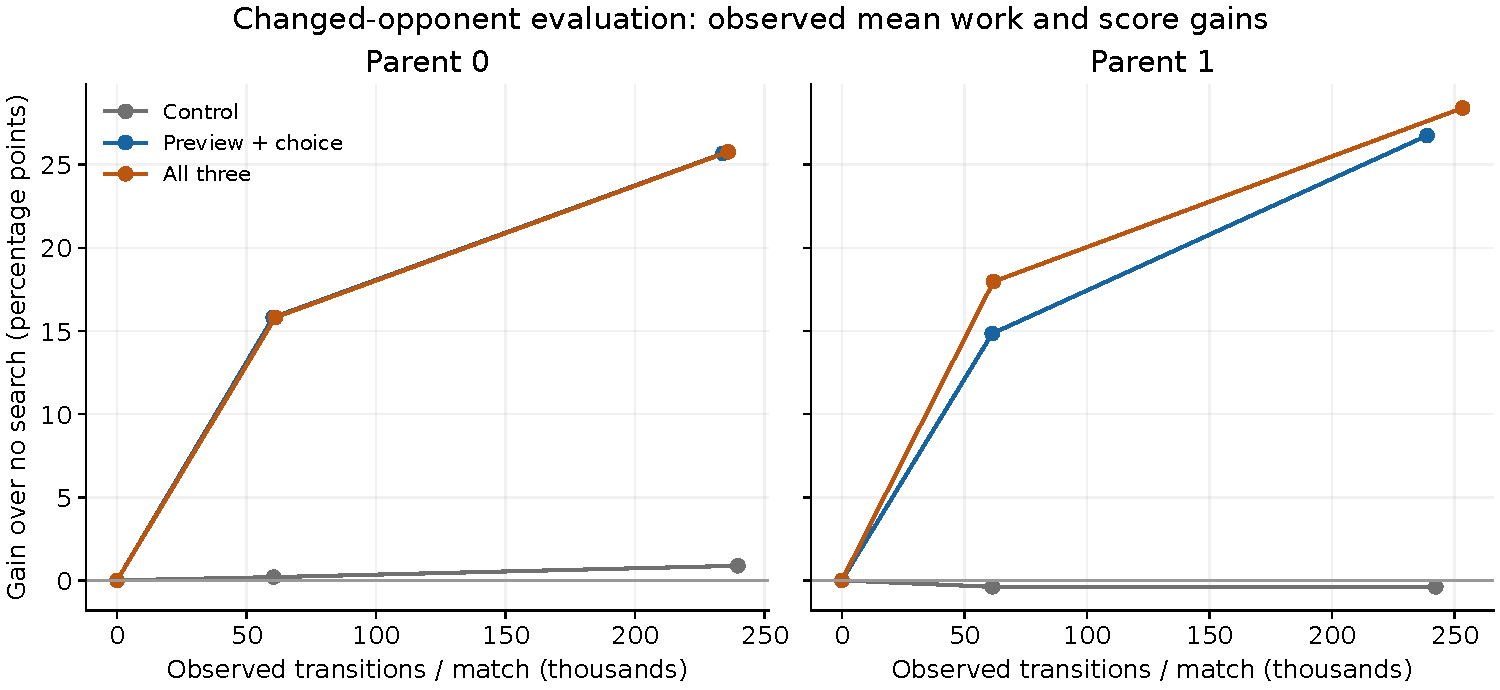
\includegraphics[width=\linewidth]{generated/public_stock_v5c/public_stock_robustness_work.pdf}
\caption{Stronger finalist actors and opponents, with retained original
control. Each curve starts at its own no-search score. Points are the three
fixed budgets at observed mean work; connecting lines do not establish a
response at untested budgets. Simultaneous comparisons are in
Table~\ref{tab:public-stock-mature-comparisons}. Adaptation budgets differ
across rules.}
\label{fig:public-stock-mature-work}
\end{figure}

\begin{table}[ht]
\centering\small
\begin{tabular}{llrrrrl}
\toprule
Rule & Parent & Target (k) & Worlds & Actual (k) & Error (\%) & Pass \\
\midrule
Control & 0 & 60 & 23 & 60.46 & +0.77 & Yes \\
Control & 0 & 240 & 91 & 239.66 & -0.14 & Yes \\
Control & 1 & 60 & 23 & 61.45 & +2.41 & Yes \\
Control & 1 & 240 & 91 & 242.32 & +0.97 & Yes \\
Preview + choice & 0 & 60 & 10 & 60.24 & +0.40 & Yes \\
Preview + choice & 0 & 240 & 39 & 233.85 & -2.56 & Yes \\
Preview + choice & 1 & 60 & 10 & 61.32 & +2.19 & Yes \\
Preview + choice & 1 & 240 & 39 & 238.77 & -0.51 & Yes \\
All three & 0 & 60 & 13 & 61.10 & +1.84 & Yes \\
All three & 0 & 240 & 52 & 235.93 & -1.69 & Yes \\
All three & 1 & 60 & 13 & 61.86 & +3.10 & Yes \\
All three & 1 & 240 & 54 & 253.31 & +5.54 & Yes \\
\bottomrule
\end{tabular}

\caption{All twelve reserved work checks. Target and actual work are
thousands of physical rollout transitions per match; worlds are per legal
root action. Every endpoint meets the fixed 10\% tolerance. Transition
counts exclude inference, sampling, bookkeeping and offline preparation;
this is not an equal-wall-time comparison.}
\label{tab:public-stock-mature-costs}
\end{table}

All twelve work checks pass, with deviations from $-2.56$\% to $+5.54$\%.
Both finalists therefore meet the prespecified matched-work criterion.
Their paired gain differences remain unresolved: preview minus all three
is $-0.10$ points with interval $[-9.21,8.79]$ for parent 0 and $-1.66$
with $[-10.35,7.23]$ for parent 1. Neither a ranking nor equivalence follows.
V4's failed work criterion remains unchanged; this separate cohort does not
retroactively repair it. Differences from V4 cannot be attributed to learning
alone because actors, opponents, tables, budgets and cohorts all differ.
The result identifies two supported routes to greater computation value,
without establishing a globally optimal rule or universally maximal strength.
\FloatBarrier
